\documentclass[tikz, border=5pt]{standalone}
\usetikzlibrary{arrows.meta, shapes, positioning, decorations.pathmorphing, patterns}

\tikzset{
  spring/.style = {
    decoration = {aspect=0.3, segment length=2mm, amplitude=2.5mm, coil, pre length=4mm, post length=3mm},
    decorate
  }
}

\begin{document}

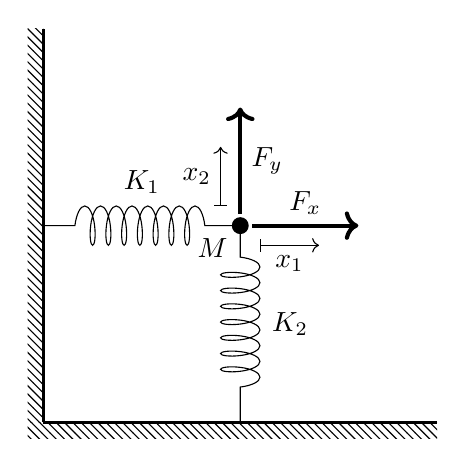
\begin{tikzpicture}

  % Walls
  \draw[thick] (0,0) -- (5,0);
  \draw[thick] (0,0) -- (0,5);
  \fill[pattern = north west lines] (0,0) rectangle (-0.2,5);
  \fill[pattern = north west lines] (-0.2,-0.2) rectangle (5,0);

  % Mass
  \draw[fill=black] (2.5, 2.5) circle (0.1) node[xshift=-10, yshift=-8] {\(M\)};

  % Springs
  \draw[spring] (0,2.5) -- (2.5,2.5) node[midway, above, yshift=8] {\(K_1\)};
  \draw[spring] (2.5,2.5) -- (2.5,0) node[midway, right, xshift=8] {\(K_2\)};

  % Displacements
  \draw[|->] (2.75,2.25) -- node[below] {\(x_1\)} (3.5,2.25);
  \draw[|->] (2.25,2.75) -- node[left] {\(x_2\)} (2.25, 3.5);

  % Forces
  \draw[->, line width=1.5pt] (2.65,2.5) -- (4,2.5) node[midway, above] {\(F_x\)};
  \draw[->, line width=1.5pt] (2.5,2.65) -- (2.5,4) node[midway, right] {\(F_y\)};

\end{tikzpicture}

\end{document}
